\section{Solutions}
\label{sec:sol}

\noindent Based on what we discussed about the difficulties in previous section, there are some solutions that came up with multiple cross-chain projects. They will be illustrated in following paragraphs.
\subsection{Ensure the atomic of transactions}

\subsubsection{Atomic swaps}
\noindent An atomic cross-chain swap\cite{herlihy2018atomic} is the basic theoretical framework for multiple parties exchange assets across multiple blockchains. Atomic operations in computer science ensures every exchange either success or failure, no third intermediate state.\\
\noindent For a more intuitive introduction to the atomic swap protocol, we assume an exchange scenario:
   \begin{figure}[H]
    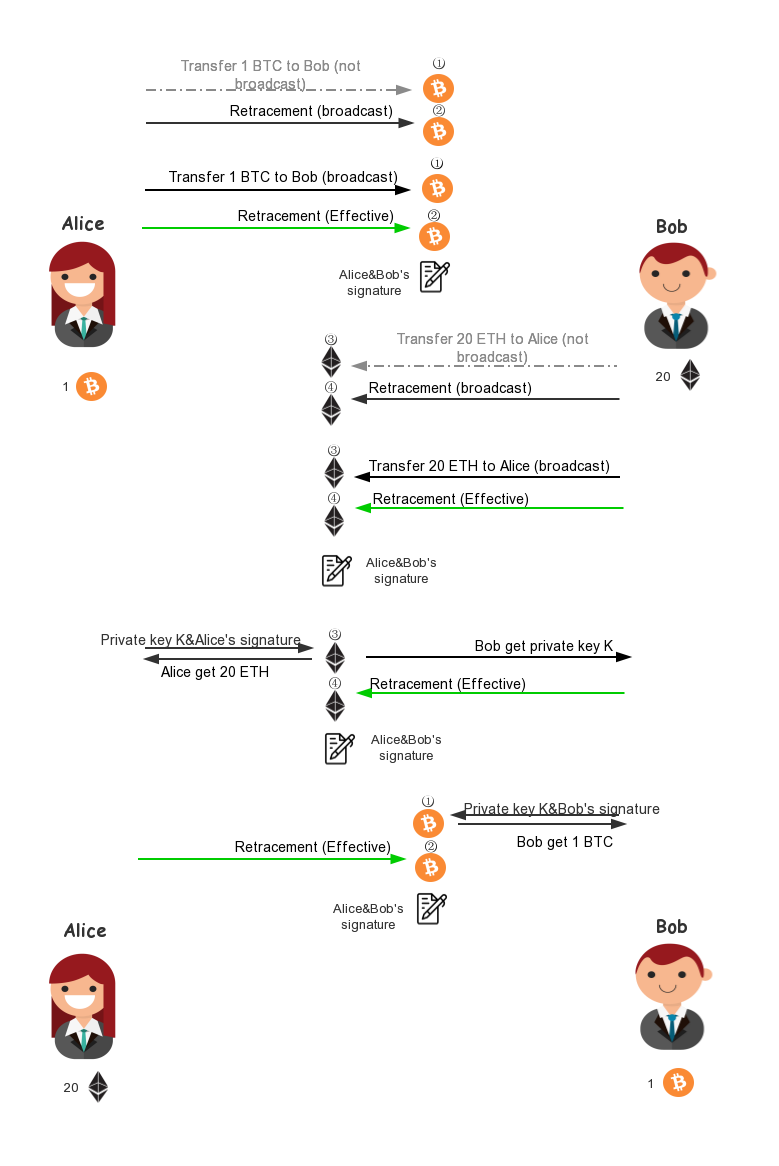
\includegraphics[width=0.79\textwidth]{./figures/atomic_swaps.png}
	\centering
    \caption{Atomic swaps diagram}%\protect\footnotemark}
    \centering
    \label{fig:atomic}
    \end{figure}
\begin{enumerate}
  \item Assume Alice has 1 BTC on chain A while Bob has 20 ETH on chain B, and Alice wants to change Bob's 20 ETH with one BTC. Both Alice and Bob have wallet addresses on both chains A and chain B.
    \item In order to initiate this transaction, Alice needs to randomly generates a key K, which is known only to Alice and then initiates a 1 BTC on chain A transaction (transaction \textcircled{1}) to Bob. The transaction can be only finished when obtains the signature of Bob and provides the key K.
    \item Before broadcast transaction \textcircled{1}, Alice will first broadcast a retracement (transaction \textcircled{2}). If transaction \textcircled{1} does not receive the correct key and signature within 48 hours, the amount paid by that will be returned to Alice. Transaction \textcircled{2} must be signed by Alice and Bob after the broadcast to take effect. At the same time, Alice will only broadcast the transaction \textcircled{1} to the network if transaction \textcircled{2} is successfully validated.
    \item Bob now sees the transaction \textcircled{2} sent by Alice. If Bob agrees, he will sign the transaction \textcircled{2}, of course, Alice will also complete the signature so that the retracement will take effect. Then Alice will broadcast the transaction \textcircled{1} to the whole network.
    \item Bob can only get the value K after he pays Alice with 20 ETH. Hence Bob initiates transaction \textcircled{3} on chain B to pay Alice 20 ETH. These 20 ETH are only available if Alice enters the decrypted key K and attaches Alice's signature. To prevent Alice from denying, Bob also issues a retracement transaction \textcircled{4} that requires Alice and Bob to sign together before the broadcast transaction \textcircled{3}, when Alice does not provide the correct key or the signature within 24 hours. then activate the retracement,20 ETH will be returned to Bob.
    \item After Alice sees the transaction \textcircled{4}, both Alice and Bob need to attach their signature to this transaction to take effect. At this time, Bob will broadcast transaction \textcircled{3} to network.
    \item In order to get 20 ETH, Alice will sign transaction \textcircled{3} with the correct value K. For now, transaction \textcircled{3} succeeds, Alice obtains 20 ETH, and Bob obtains key K.
    \item After Bob gets the key K, he goes back to chain A, enters the key K and his signature, and finally gets 1 BTC from Alice.
\end{enumerate}
\noindent From the diagram, we could obtain that the atomic swap protocol does not transfer the assets of Chain A to Chain B, but only the assets ownership of both chains. The total assets of Chain A and Chain B have not changed, so it can only achieve asset exchange between chains and cannot achieve asset transfer.\\
\noindent This solution not only can be applied to the decentralized ledger system, but also to the centralized ledgers. As long as the two systems provide the functions of retracement, time lock, and key lock.

\subsubsection{Hash Time-Locked Contracts(HTLC)}
\noindent HTLC is a very technical implementation of the atomic swap protocol. It guarantees the atomicity of the transaction through the hash lock and the time lock mechanism. In different systems, whether it is a blockchain system or a centralized ledger system, despite the ways of implementing the lock, the principle behind it is the same, that is, only certain hash conditions or time met, the transaction is allowed to take effect.

        \begin{figure}[H]
        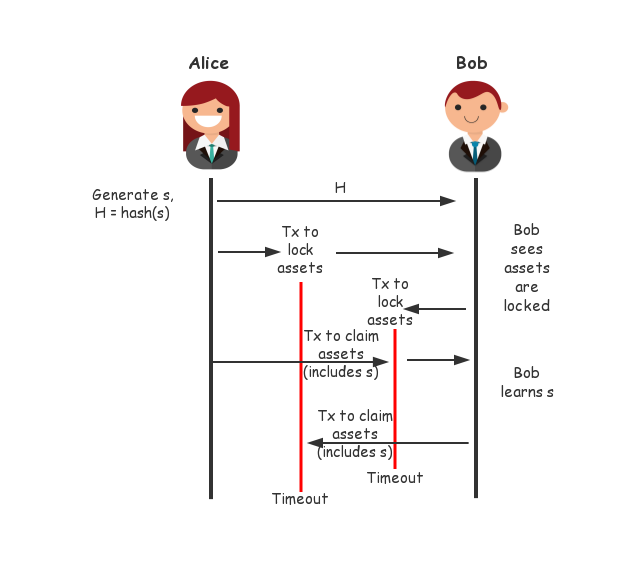
\includegraphics[width=0.8\textwidth]{./figures/Hashlock.png}
        \centering
        \caption{Hash Time-lock Contract diagram}%\protect\footnotemark}
        \centering
        \label{fig:hash}
        \end{figure}
\noindent Using only hash time locks is not enough when you want to achieve cross-chain asset transfer, you also need to cooperate with other cross-chain technologies to ensure the authenticity of cross-chain transactions.


\subsubsection{Hash Time-locked Agreements(HTLA)}
\noindent HTLA is one HTLC generalization protocol came up by Interledger\cite{HTLA}, regardless whether the system support HTLC or not, whether it's a distributed or centralized ledger. HTLA can be used to implement cross-chain exchange between system or even support multi-hop cross-chain interchange between multiple systems, as shown in the Figure \ref{fig:HTLA} below.
   \begin{figure}[H]
    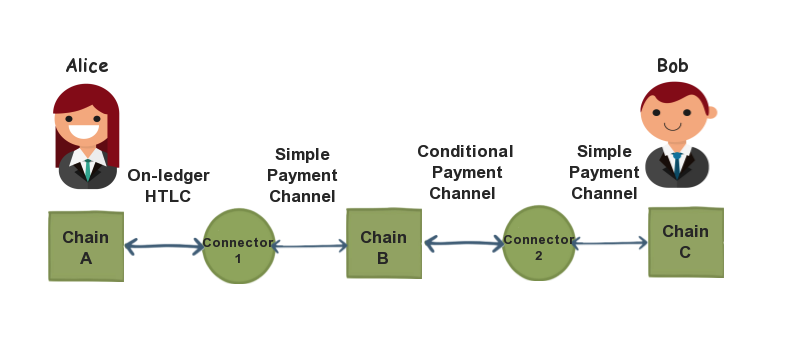
\includegraphics[width=0.8\textwidth]{./figures/HTLA.png}
    \centering
    \caption{Interledger HTLA diagram}%\protect\footnotemark}
    \centering
    \label{fig:HTLA}
    \end{figure}
    
\noindent Alice and Bob can across between blockchains A, B, and C via HTLA, and each blockchain supports different cross-chain protocols. The connector here plays a role in connection and isolation. Linking blockchains that support different cross-chain protocols together, and again isolate them, so that blockchains do not interfere with each other.\\
\noindent HTLA supports multiple cross-chain protocols based on HTLC, some of them are mentioned in Figure \ref{fig:HTLA}.


\subsection{Complete the transaction confirmation}
\noindent As we all know, blockchain systems are relatively independent and closed, there's no direct communication way for them to confirm every piece of records that happened. So no matter how it evolves, there will always be a ``middle-man'' between the two chains, taking on the role of information exchange between the two chains.\\
\noindent Here the ``middle-man'' represent any entity that could interact with two chains, it may be one or a group, maybe the centralized or distributed agency, maybe a separate chain or even a functional module. The ``middle-man'' usually acts as a node for two blockchains at the same time, so that only one application software can be deployed on the same node to obtain the others' system data.\\
\noindent After the ``middle-man'' completes the data collection, how to confirm the transaction, where to confirm, and who confirms becomes the key point of this problem. According to different schemes, this process can be summarized in three ways:
\begin{itemize}
    \item \textbf{Notary\cite{buterin2016chain}}:\\
    In the notary scheme, a trusted one or group is used to declare to the chain X that an event has occurred on the chain Y, or that the statement is correct. These groups can both automatically or requested to listen and respond to events. There are 3 different child-schemes came up in the evolution of this model: 
    \begin{itemize}
        \item \texttt{Centralized Notary schemes}\\
        The centralized notary mechanism is also called the single-signature notary mechanism, usually played by a single designated independent node or institution, which is the simplest mode. Its purpose is instead of letting Alice and Bob, two strange individuals deal, it's not as reliable as indirect transactions with third-party institutions with credit endorsements (such as Alipay). Since Alice and Bob exist in different ledger systems, the notary is technically required to be compatible with two or more systems at the same time.
        \begin{figure}[H]
        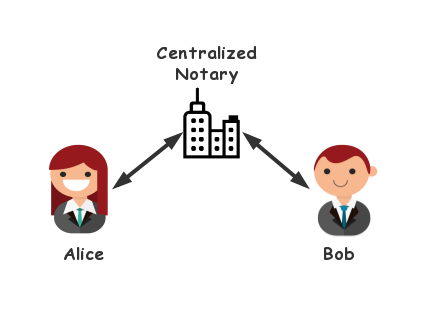
\includegraphics[width=0.7\textwidth]{./figures/cnotary.png}
        \centering
        \caption{Centralized Notary Scheme diagram}%\protect\footnotemark}
        \centering
        \label{fig:cno}
        \end{figure}
        To some extent, the use of centralized institutions has replaced technical credit guarantees, from technical credibility to traditional credit intermediaries. Although this kind of mode has fast transaction processing, strong compatibility, and simple technical architecture, the security of the central node has become a key bottleneck for system stability.
        
        \item \texttt{Multi-sig Notary schemes}\\
       The multi-signature notary mechanism is accomplished by multiple notaries that can sign a common agreement on their respective ledgers to complete the cross-chain transaction. Each node of the multi-signature notary group has its own key, and cross-chain transactions can only be confirmed when a certain number or proportions of notary signatures are reached.

        \begin{figure}[H]
        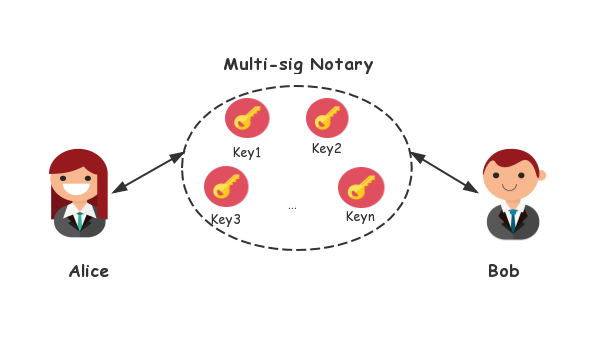
\includegraphics[width=0.8\textwidth]{./figures/mnotary.png}
        \centering
        \caption{Multi-sig Notary Scheme diagram}%\protect\footnotemark}
        \centering
        \label{fig:mno}
        \end{figure}
       This method is more secure than the single-signature mode, and a few notaries who are attacked or do evil will not affect the normal operation of the system. However, this approach requires both chains to have the ability to support multiple signatures.
        \item  \texttt{Distributed signature Notary schemes} \\
        The main difference between distributed signature and multi-signature is the signature generation. Distributed signature using \textit{Multi-Party Computation}(MPC), which will enhance the security as well as the implementation difficulty.
        \begin{figure}[H]
        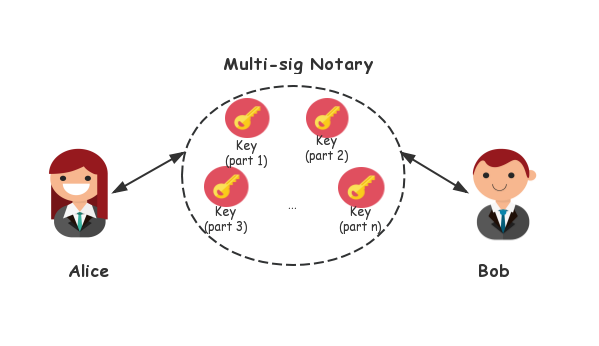
\includegraphics[width=0.8\textwidth]{./figures/dnotary.png}
        \centering
        \caption{Distributed signature Notary Scheme diagram}%\protect\footnotemark}
        \centering
        \label{fig:dno}
        \end{figure}
        As Figure \ref{fig:dno} shows, distributed signature based on cryptography, the key point is that for cross-chain transactions, the system generates one and only one key, and no one in the notary group will have a complete key. The key is randomly sent to each notary node in the form of fragments.
        Meanwhile, the fragment is the processed ciphertext, so even if all the notaries put together the pieces, the complete key cannot be known, and the security of the key is fully guaranteed.
    \end{itemize}
    \item \textbf{Relay\cite{buterin2016chain}}:\\
    Relay is one flexible and easy-to-expand cross-chain technology that does not rely on trusted third parties to help with transaction verification. Instead, it is self-verified by the receiving chain after receiving the send chain data. Self-verification methods are depending on the system structure. For example, BTC-relay\cite{btc-relay} based on \textit{Simplified Payment Verification}(SPV), and Cosmos\cite{cosmos} rely on verify the number of nodes' signature.\\
    \textsc{Vitalik} mentioned Relay in his Chain Interoperability paper\cite{buterin2016chain}, pointing out that chain A and chain B can use the other party's block data for information synchronization and cross-chain calls. Currently, information synchronization can be done, but there is no mature technical solution for cross-chain calls. Two chains cannot verify the validity of each others block at the same time, otherwise, they will fall into an infinite loop of nesting. If chain A owns the block data of chain B, then chain A needs to be confirmed in the case of chain B transaction confirmation, and chain B needs to wait for chain A's transaction confirmation because it also has block A's block data, it goes on as a loop.
    
    
    
    \item \textbf{Sidechains}:\\
     The concept of a sidechain as defined in white paper\cite{back2014enabling} is: \textit{sidechain is a blockchain that validates data from other blockchains}. However, this explanation was considered to be too broad and not rigorous by \textsc{Vitalik Buterin} in \textsc{Chain Interoperability}\cite{buterin2016chain}. ``Sidechain'' is more frequently used to refer to what Blockstream calls a ``pegged sidechain'', where the functionality of a blockchain is of an anchored asset of another asset, which chain is regarded as the parent chain. In this way, this relationship is based on assets, not the blockchain itself. This is a strong coupling cross-chain structure using directly embeds part of the data of the original chain into its own block or storage space. In the case of cross-chain transactions,  verification can be completed directly through the original chain data stored in the system. This method is generally considered bidirectionally at the beginning of the system design.\\
     Compared to notary and relay, the sidechain is more direct. The state of one chain will be directly reflected in the data of the other chain. When one chain is attacked, the other chain may also be affected. This model is more suitable for the design of the same system, which allows the two sides to become a whole without losing the relative independence of the ledgers.

\end{itemize}
\subsection{Realize multiple chains interoperability}
\noindent The computer network connects the original independent computers into a local area network, the local area network develops into a metropolitan area network, the metropolitan area network evolves into the Internet, and the Internet connects the people of the world like never before.\\
\noindent However, for the emerging technology/industry of blockchain, it is still in the ``single-machine'' era, and the interactions demand between chains and chains will become increasingly strong with the application of blockchain.\\
\noindent To realize interoperability among multiple chains, there are two potential aspects of difficulties that need to overcome: 
\begin{itemize}
    \item How to achieve interoperability among blockchains system that has already developed.
    \item How to prepare/setup the way for the interconnections among the new blockchains in the future.
\end{itemize}

\subsubsection{Active compatibility}
\noindent This solution is mainly aimed at the existing blockchain system. First, there are different blockchain application systems in the upper layer, and then the underlying cross-chain mechanism is developed.\\
\noindent Usually these systems are heterogeneous chains and need to be docked one by one, but there is also a different solution for a pair of connections.
\begin{enumerate}
    \item Direct interconnection between the two chains
        \begin{figure}[H]
        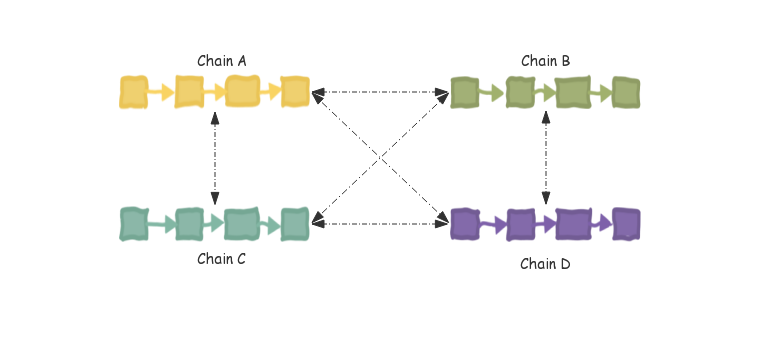
\includegraphics[width=1\textwidth]{./figures/direct.png}
        \centering
        \caption{Direct interconnection network architecture diagram}
        \centering
        \label{fig:direct}
        
        \end{figure}
    This method is the most time-consuming and laborious without the support of the unified underlying protocol. It is necessary to establish 6 paths between the 4 chains to realize the interconnection between them. And each path needs to be customized. Although this method is not scalable, it can guarantee better security and independence. Once an attack occurs, it is difficult to affect the entire network.
    \item Third-party cross-chain platform
      \begin{figure}[H]
        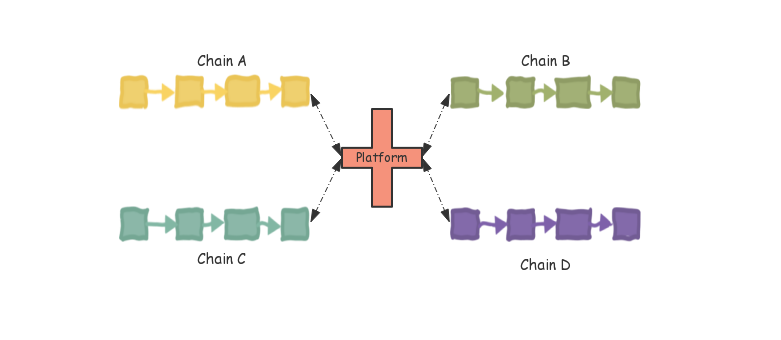
\includegraphics[width=1\textwidth]{./figures/platform.png}
        \centering
        \caption{Cross-chain platform network architecture diagram}
        \centering
        \label{fig:platform}
        
        \end{figure}
    To establish a cross-chain platform, blockchains can indirectly interconnect with each other. Thus, only 4 paths are required to build a cross-chain network. However, in this method, the cross-chain platform will become the key point and performance bottleneck of the entire cross-chain network (not necessarily the bottleneck, but it may be in the future). Once the cross-chain platform is attacked, the entire cross-chain network will be paralyzed.
\end{enumerate}
\subsubsection{Passive compatibility}
\noindent Passive compatibility is mainly aimed at the blockchain system that has not been developed. It first builds the underlying cross-chain platform, allowing other blockchain systems to be easily, conveniently and securely accessed. Cross-chain platforms will prioritize the development of systems and protocol standards that apply to interoperability between the various chains. The subsequent development of standards-compliant development on existing platforms allows for the creation of blockchains that naturally have cross-chain functionality within the system. However, the cross-chain mentioned here refers to the chain that conforms to the protocol standard can be easily connected to each other. If it is to interoperate with other chains outside the system, it is necessary to develop a separate middleware to communicate.\\

\noindent In addition, different cross-chain platforms can support different types of blockchains, such as Cosmos supporting isomorphic chains and Polkadot supporting heterogeneous chains, both of which are highly scalable, and will be later discussed in Section \ref{sec:p}.